\section{Single particle heat transfer}

\begin{figure}[t]
	\centering
	\caption{Each ceramic pebble in a fusion reactor will experience multiple modes of heat transfer.}
	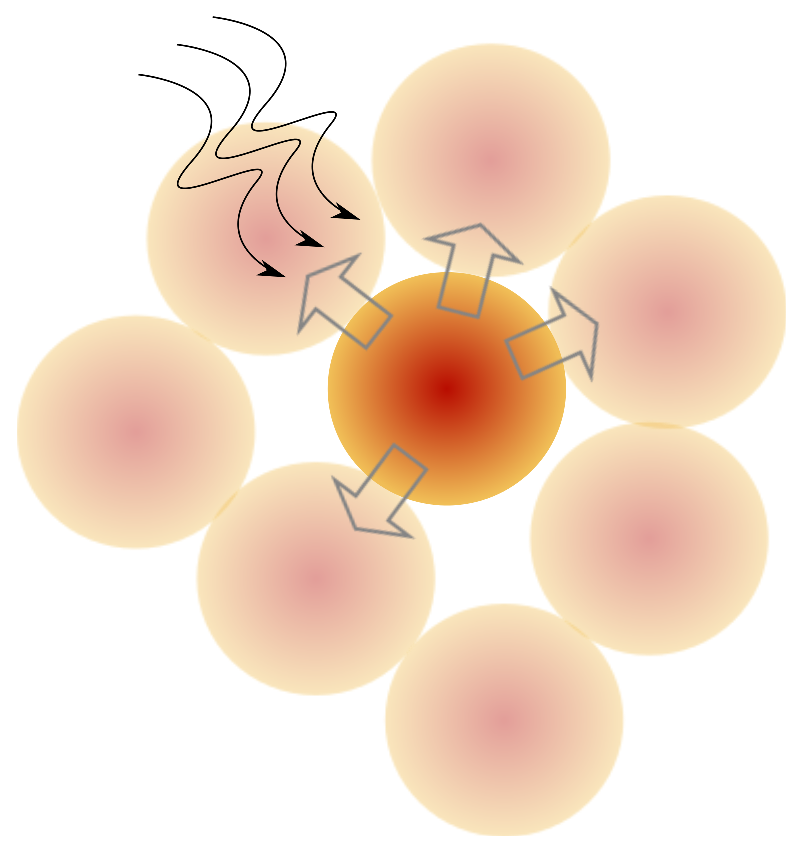
\includegraphics[width=0.75\textwidth]{chapters/figures/pebble-complete-heat-transfer}\label{fig:peb-comp-ht}
\end{figure}

Shown in Fig.~\ref{fig:peb-comp-ht} are all the modes of energy transfer on a pebble inside the fusion reactor. There is:

\begin{enumerate}
\item energy generated internal to the pebble caused by nuclear heating,
\item conduction internally of the solid material to the surface of the pebble, 
\item conduction between neighboring pebbles at their areas of contact, 
\item radiation between neighboring solids, and 
\item convective heat transfer with the interstitial helium gas (which includes energy carried far downstream or redeposited to neighboring pebbles).
\end{enumerate}









\subsection{Nuclear heating}

Nuclear deposition of energy is handled in a straightforward manner in the DEM computations with a simple source term on the energy balance equation. 












\subsection{Conduction through the solid}\label{sec:ht-pebble-conduction}

The importance of internal conduction of the solid depends on both the rate of convective heat transfer with the fluid as well as conductive heat transfer to neighbors. To quantify the negligibility of internal conduction relative to surface convection, we look at the Biot number of the particles in our system. The Biot number is a ratio of

\begin{equation}
	\Bi = \frac{\text{Rate of convective heat transfer from surface}}{\text{Rate of internal conduction to surface}} = \frac{hd_p}{k_s}
\end{equation}

or in terms of the Nusselt number,

\begin{equation}
	\Bi = \Nu \frac{k_f}{k_s}
\end{equation}

where $h$ is the average heat transfer coefficient, $d_p$ is the particle diameter, $k_f$ is the conductivity of the passing fluid, and $k_s$ is the bulk conductivity of the solid. When the $\Bi \ll 1$, the material is considered isothermal and internal conduction is safely ignored. 

The helium purge gas moving through the packed beds is not intended to act as a heat transfer agent and moves along at a creeping flow rate. Therefore, for a first approximation we assume the Nusselt number is $\Nu = 2$. This leads to the requirement that

\begin{equation}
	2 \frac{k_f}{k_s} \ll 1
\end{equation}

The conductivity of helium over the temperature range of 300 to 800 $^\circ$C is approximately 0.3 \si{W/m-K}. The solid conductivity of \lit and \lis are approximately 2 \si{W/m-K}. Because of the low conductivity of our solid, the Biot assumption is barely valid, $0.3 < 1$. 

[Go back through Batchelor and O'Brien~\cite{Batchelor1977} paper]

\begin{equation}
	\frac{ k_s }{ k_f } \frac{a}{R^*} = \lambda
\end{equation}

Similar to the lumped capacitance assumptions, if $\lambda \gg 1$, the solid is approximately is isothermal. The second group on the left-hand side of this condition we remember from the assumptions of Hertz theory, where we require $\frac{a}{R^*} \ll 1^*$. Therefore to satisfy the condition of $\lambda \gg 1$, we require very large conductivity ratios of solid to fluid, $\frac{k_s}{k_f} \gg 1$. Alternatively this is satisfied by definition if the solids exist in vacuum.

Assuming that we satisfy the condition of isothermal solids, we address the conduction between solids in their small regions of contact.

[more details]










\subsection{Particle-particle conduction}

Handling the heat transfer between contacting particles has been investigated extensively by researchers in a number of fields\cite{Zhou2009,Zhang2011,Wu2011,Vargas2001,Li2000,Chaudhuri2006}. The amount of energy per time that can be transported per difference in temperature between pebble $i$ and $j$ as a conductance $h_{ij}$. Defined as

\begin{equation}\label{eq:pebble-conductance}
	\frac{h_{ij}}{k^*}= 2\left[\frac{3F_nR^*}{4E^*}\right]^{1/3}
\end{equation}

$k^*= 2k_ik_j/(k_i+k_j)$ is the effective solid conductivity of the two particles, and $F_n$ is the magnitude of the normal force between particles $i$ and $j$ as calculated by Eq.~\ref{eq:hertzForce}. Therefore, if we consider particles at temperatures $T_i$ and $T_j$ in contact, they will transfer heat at a rate of

\begin{equation}
	Q_{ij} = h_{ij}(T_i - T_j)
\end{equation} 











\subsection{Convection}











\subsection{Particle-particle radiation}